\documentclass[a4paper, oneside, 11pt]{article}

\usepackage[english]{babel}
\usepackage[T1]{fontenc}

\usepackage[a4paper,top=2.5cm,bottom=2.5cm,left=2cm,right=2cm]{geometry}

\usepackage{amsmath}
\usepackage{graphicx}
\usepackage{fancyhdr}
\usepackage{float}
\usepackage[labelfont=bf]{caption}
\usepackage{subcaption}
\usepackage{comment}
\usepackage{lastpage}
\usepackage{siunitx}
\usepackage{csquotes}
\usepackage{amsfonts}
\usepackage{textcomp}

\usepackage{hyperref}

\pagestyle{fancy}
\fancyhf{}
\rhead{Sampling and Aliasing}
\lhead{Digital Signal Processing}
\cfoot{Page  \thepage \hspace{1pt} of \pageref{LastPage}}

\begin{document}

\begin{titlepage}
	\begin{center}
		\begin{figure}[htb!]
			\centering
				
\includegraphics[width=10cm]{figures/istlogo.jpg}
		\end{figure}
        
        \LARGE{\textbf{Instituto Superior Técnico}}\\
        \vspace{20pt}
        \Large{Integrated Masters in Aerospace Engineering}\\
        \vspace{10pt}
        \Large{Digital Signal Processing}\\
        \vspace{10pt}
        \Large{1\textsuperscript{st} Semester 2020/2021}\\
            
        \vspace{40pt}
        \noindent\rule{15cm}{1pt}\\
        \Huge{\center \textbf{Laboratory 1}} 
        \par 
        \Huge{\center \textbf{Sampling and Aliasing}}\\
        \noindent\rule{15cm}{1pt}\\
        
        \vspace{60pt}
        \large{\begin{tabular}{ll}
            \textbf{Group 40:} & \textbf{Professor:} \\
            89683, José Neves & Prof. Rita Cunha\\
            89691, Leonardo Pedroso \hspace{1cm} & \\
        \end{tabular}}
    
        \vspace{60pt}
        \large{\today}
	\end{center}
\end{titlepage}

\newpage
\pagenumbering{arabic}
\setcounter{page}{1}

\section{Introduction}

This report was written in the scope of the Digital Signal Processing course and was focused on sampling operations and aliasing phenomena. In this laboratory session, a continuous-time chirp and a sharp melody of a violin playing called \textit{Romanza} were analyzed regarding the previously mentioned aspects. Firstly, the chirp was mathematically defined, sampled and heard. The relationship between the mathematical representation and the sound heard was analyzed and its spectrogram was presented to complement that analysis. To study the aliasing phenomenon associated with this signal, a new signal was created and several sinusoidal waves were also considered at different sampling frequencies. Lastly, the melody was analysed in its original form, at a fifth of the original sampling rate, and low-pass filtered and sampled at a fifth of the original sampling rate.

\section{Continuous-time chirp}

\subsection{1.a) Relationship between the signal and the sound heard}

Let $x_c: \mathbb{R} \rightarrow \mathbb{R}$ denote a continuous-time chirp given by
\begin{equation} \label{eq:x_c}
    x_c (t) = \cos \left [ 2 \pi \left ( \frac{1}{3} k_2 t^3 + \frac{1}{2} k_1 t^2 + F_0 t + \phi_0 \right) \right],
\end{equation}
where $t$ represents the time in seconds, $k_2 = 1000 \; s^{-3}$, $k_1 = 0 \; s^{-2}$, $F_0 = \SI{0}{\hertz}$, and $\phi_0 = \SI{0}{\radian}$. Taking the time derivative of the phase of the cosine in \eqref{eq:x_c}, one can obtain the instantaneous frequency of $x_c (t)$,
\begin{equation} \label{eq:Omega}
    \Omega (t) = 2 \pi \left (k_2 t^2 + k_1 t + F_0 \right).
\end{equation}
From \eqref{eq:Omega}, it is possible to verify that, since $k_2$ is positive and $k_1 = 0$, the instantaneous frequency of $x_c$ is always increasing. Given it is always increasing, it varies monotonically, and, therefore, $x_c (t)$ is indeed a chirp.

The signal $x_c (t)$ can be sampled into a discrete-time signal. Given a sampling frequency of $f_s = \SI{8000}{\hertz}$ and sampling it in the interval $[0,2] \si{\second}$, the sampled signal, $x(n)$, can be obtained as
\begin{equation} \label{eq:x}
    x (n) = x_c (n T), \text{ for } n = 0, ..., 2 f_s,
\end{equation}
where $T = 1/f_s$ is the sampling period.

The signal $x_c$ may be interpreted as a sound wave and be produced and heard as was executed in this laboratory session through the MATLAB{\texttrademark} command \texttt{soundsc}. The signal $x_c(t)$ is just a sinusoid with instantaneous frequency $\Omega (t)$ and $\Omega (t)$ is an always increasing quadratic function with positive second derivative. Therefore, it was expected that the sound produced would begin at zero frequency and increase its frequency at an increasing rate. In a more practical sense, the frequency of a sound determines how high-pitched it is, \textit{i.e.}, a sound with an higher frequency is higher-pitched than one with a lower frequency. Hence, it was expected that the sound produced would be very low-pitched in the beginning and get higher-pitched at an increasing rate from there on. Upon hearing the sound produced, it was clear that these assumptions were in fact correct. On the other hand, it also appeared that, at this sampling rate, the signal was not distorted since it followed the tendency given by the instantaneous frequency given in \eqref{eq:Omega}. From the Nyquist or Sampling Theorem, it is possible to state, given \eqref{eq:Omega}, that the highest frequency of $x_c(t)$ is $\SI{4}{\kilo \hertz}$ and, thus, the minimum sampling frequency to avoid distortion is $f_{s\:\mathrm{min}} = 2\times \SI{4}{\kilo \hertz} = \SI{8}{\kilo \hertz}$. After some experiments with decreasing sampling frequency values, it was possible to distinguish some clear distortion in the sound at $\SI{6000}{\hertz}$ and the end of the time interval, since it suddenly begins to be lower-pitched at that point. Since $\SI{6000}{\kilo \hertz} < \SI{8000}{\kilo \hertz}$, one can state that these experiments are in accordance with the Sampling Theorem.

\subsection{2.b) Relationship between the spectrogram and the sound heard}

In the laboratory session, the spectrogram of the signal $x(n)$ defined in \eqref{eq:x} was obtained with the MATLAB{\texttrademark} command \texttt{spectrogram} for an Hanning window with length $N = 320$, $3N/4$ overlapped samples, $4 N$ DFT points, and sampling frequency $f_s = \SI{8000}{\hertz}$. It is represented in Fig. \ref{fig:spectrogram_x}. The spectrogram relates power per frequency to various values of frequency smaller than the Nyquist frequency of the signal and throughout the duration of the signal. This spectrogram was chosen between various others with different values of window lengths since it was the sharpest one obtained. Comparing this figure with \eqref{eq:Omega}, it is possible to observe that the frequencies with the most power per frequency over time follow a parabola coincident with the one created by the instantaneous frequencies of the signal, which was expected. Similarly to what was written in the previous section, it is possible to observe that over time the frequencies with the most power per frequency are increasing at an increasing rate and that in the beginning the most powerful frequency was $\SI{0}{\kilo \hertz}$. Given the high-pitched to high frequency and low-pitched to low frequency correspondence already mentioned, the sound produced, which was low-pitched in the beginning and becoming higher-pitched at an increasing rate, is in accordance to the represented spectrogram.

\begin{figure}[h!]
    \centering
    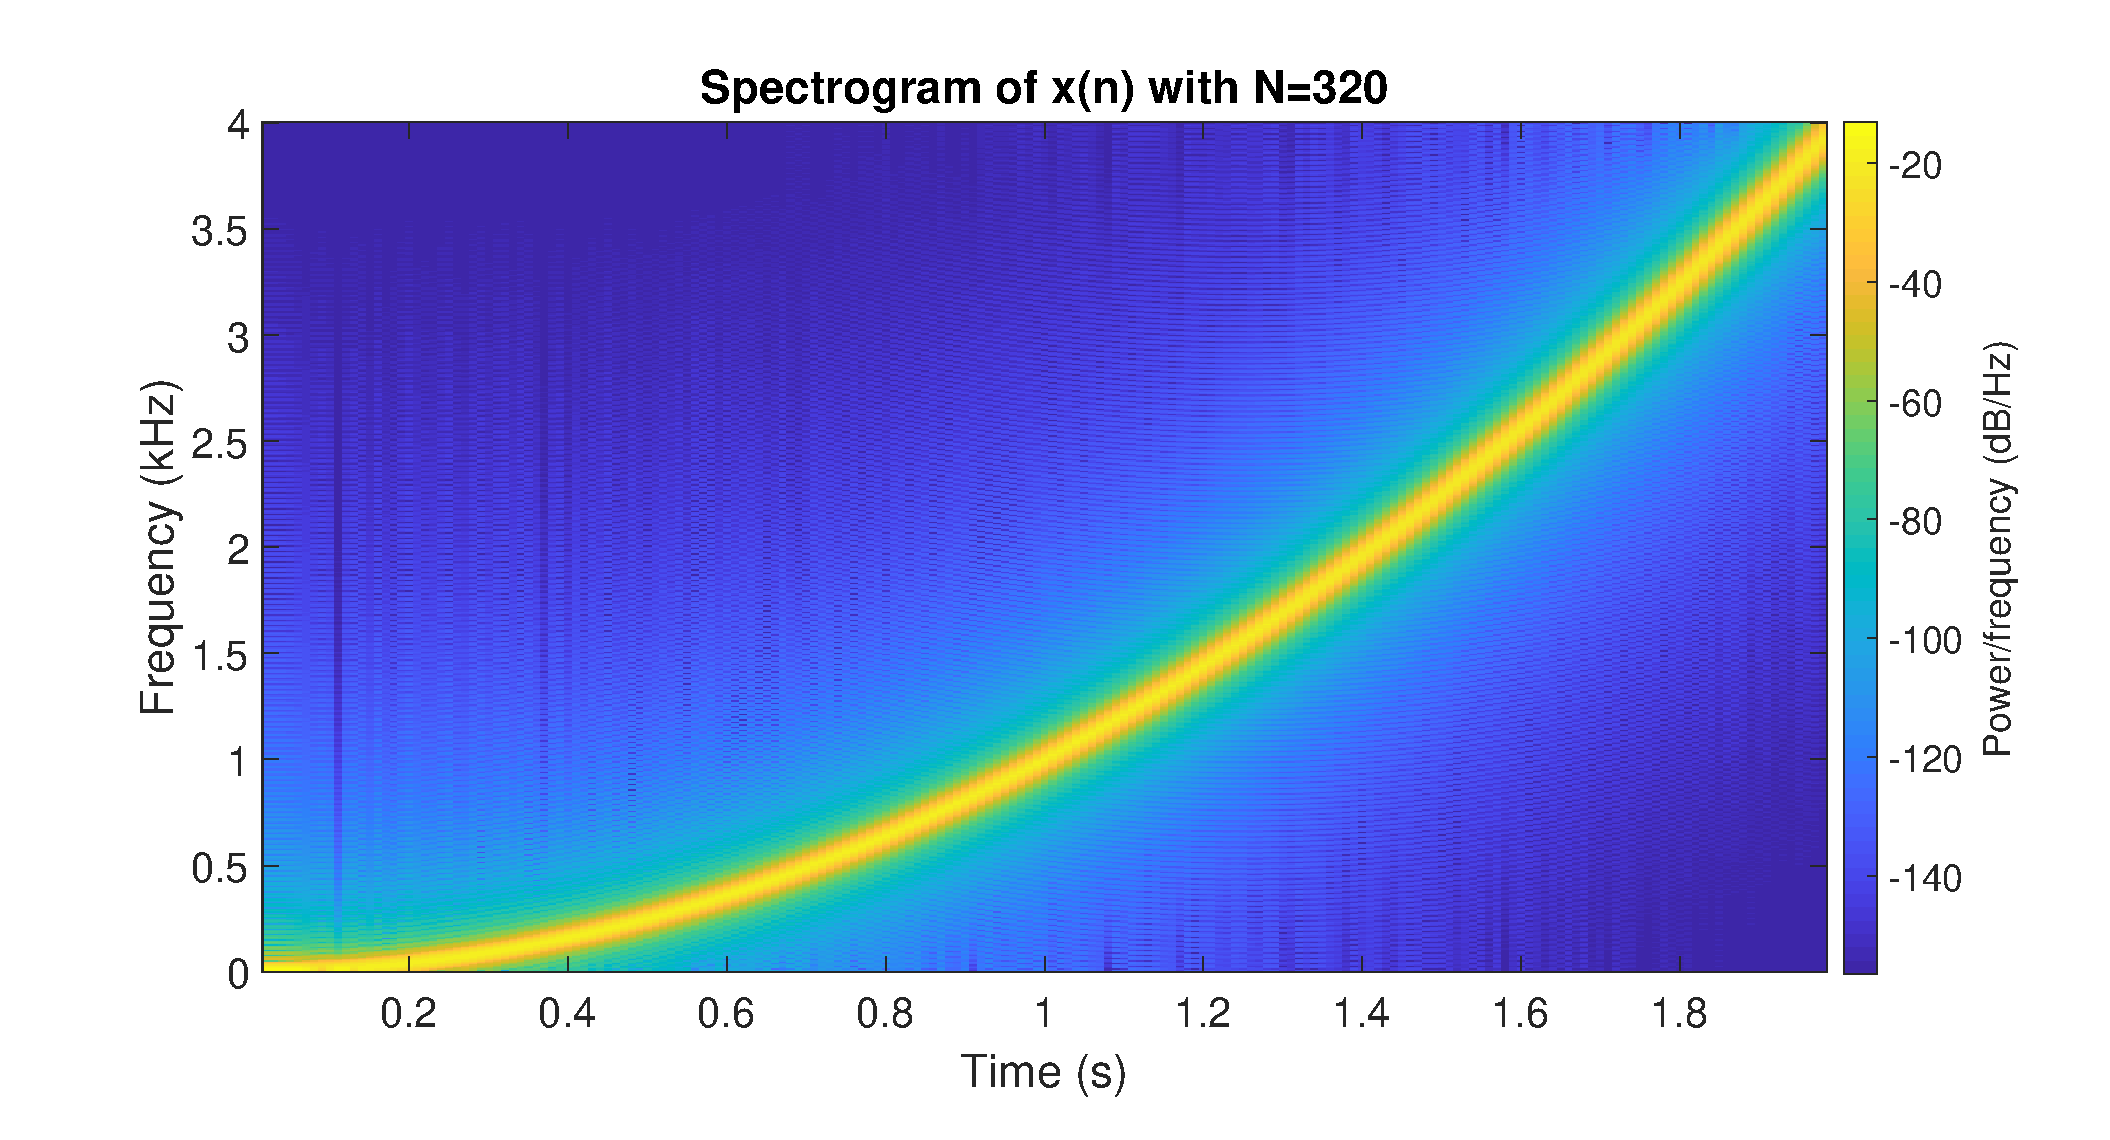
\includegraphics[width = 0.8 \textwidth]{figures/spectrogram_x.pdf}
    \caption{Spectrogram of $x(n)$ obtained with the MATLAB{\texttrademark} command \texttt{spectrogram} for an Hanning window with length $N = 320$, $3N/4$ overlapped samples, $4 N$ DFT points, and sampling frequency $f_s = \SI{8000}{\hertz}$.}
    \label{fig:spectrogram_x}
\end{figure}

\subsection{3.a) Sampling frequency of the newly defined signal}

From $x(n)$, it is possible to define a new signal $y(n)$ such that
\begin{equation} \label{eq:y}
    y(n) = x(2 n).
\end{equation}
In order to determine the sampling frequency of $y(n)$, one can write from \eqref{eq:x} and \eqref{eq:y},
\begin{equation}
    y (n) = x_c \left (2 \frac{n}{fs} \right) = x_c \left (\frac{n}{f_s/2} \right),
\end{equation}
concluding, by comparison, that the sampling frequency of $y(n)$ shall be $f_s/2 = \SI{4000}{\hertz}$. It was also possible to come to this conclusion by observing that for every two samples of $x(n)$ there will only be one sample of $y(n)$.
    
\subsection{3.b) Analysis of the newly defined signal}

For the signal $y(n)$, a spectrogram was also created in the same fashion but with its own sampling frequency, $f_s/2$, and with a different window length. The new window length, $N_y$, was chosen so that the window duration remained the same. Denoting the window duration by $\Delta T$, one can write for the window duration of $x(n)$, $\Delta T_x = N / f_s$, which means that for $\Delta T_y = \Delta T_x$, $N_y = N/2$. The spectrogram of $y(n)$ is represented in Fig.~\ref{fig:spectrogram_y}. Comparing the two presented spectrograms, one may observe that they are coincident from the beginning to approximately $\SI{1.4}{\second}$, when the instantaneous frequency of $x_c(t)$ is approximately $\SI{2}{\kilo \hertz}$. It is important to remember that it was already observed for the signal $x(n)$ that the instantaneous frequencies of $x_c(t)$ are coincident with the most powerful frequencies of $x(n)$. From there on, the most powerful frequencies of $y(n)$ start to decline over time reaching 0 at the end of the represented time interval. This is in accordance to what is heard. First the sound follows the trend of $x(n)$ going from low-pitched to high-pitched at an increasing rate and then suddenly it starts to become lower-pitched until it is very low-pitched. Since the original signal had an always increasing instantaneous frequency, it is obvious that the signal $y(n)$ is distorted.

To explain this behavior, one starts by pointing out that the two spectrograms are coincident until half the sampling frequency of $y(n)$. According to the Nyquist or Sampling Theorem, this would be expected. This theorem states that a signal can only be sampled without distortion or aliasing if its sampling frequency is double of the highest frequency of the sampled signal which is the case of the signal $y(n)$ in the initial part of the interval. In fact, taking into consideration \eqref{eq:Omega} and the value of the final instant of the interval, it is clear that the highest frequency of $x_c(t)$ is $\SI{4}{\kilo \hertz}$, which means that only sampling frequencies larger than $\SI{8}{\kilo \hertz}$ are suited to sample $x_c(t)$. That is why in $x(n)$ there is no distortion. Even though the Sampling Theorem establishes which sampling frequencies cause distortion or not, it does not state what happens when there is distortion. In Fig. \ref{fig:spectrogram_y}, it is observed that larger continuous frequencies are mapped into smaller frequencies after sampling but this effect will be further analyzed in the next section.

\begin{figure}[h!]
    \centering
    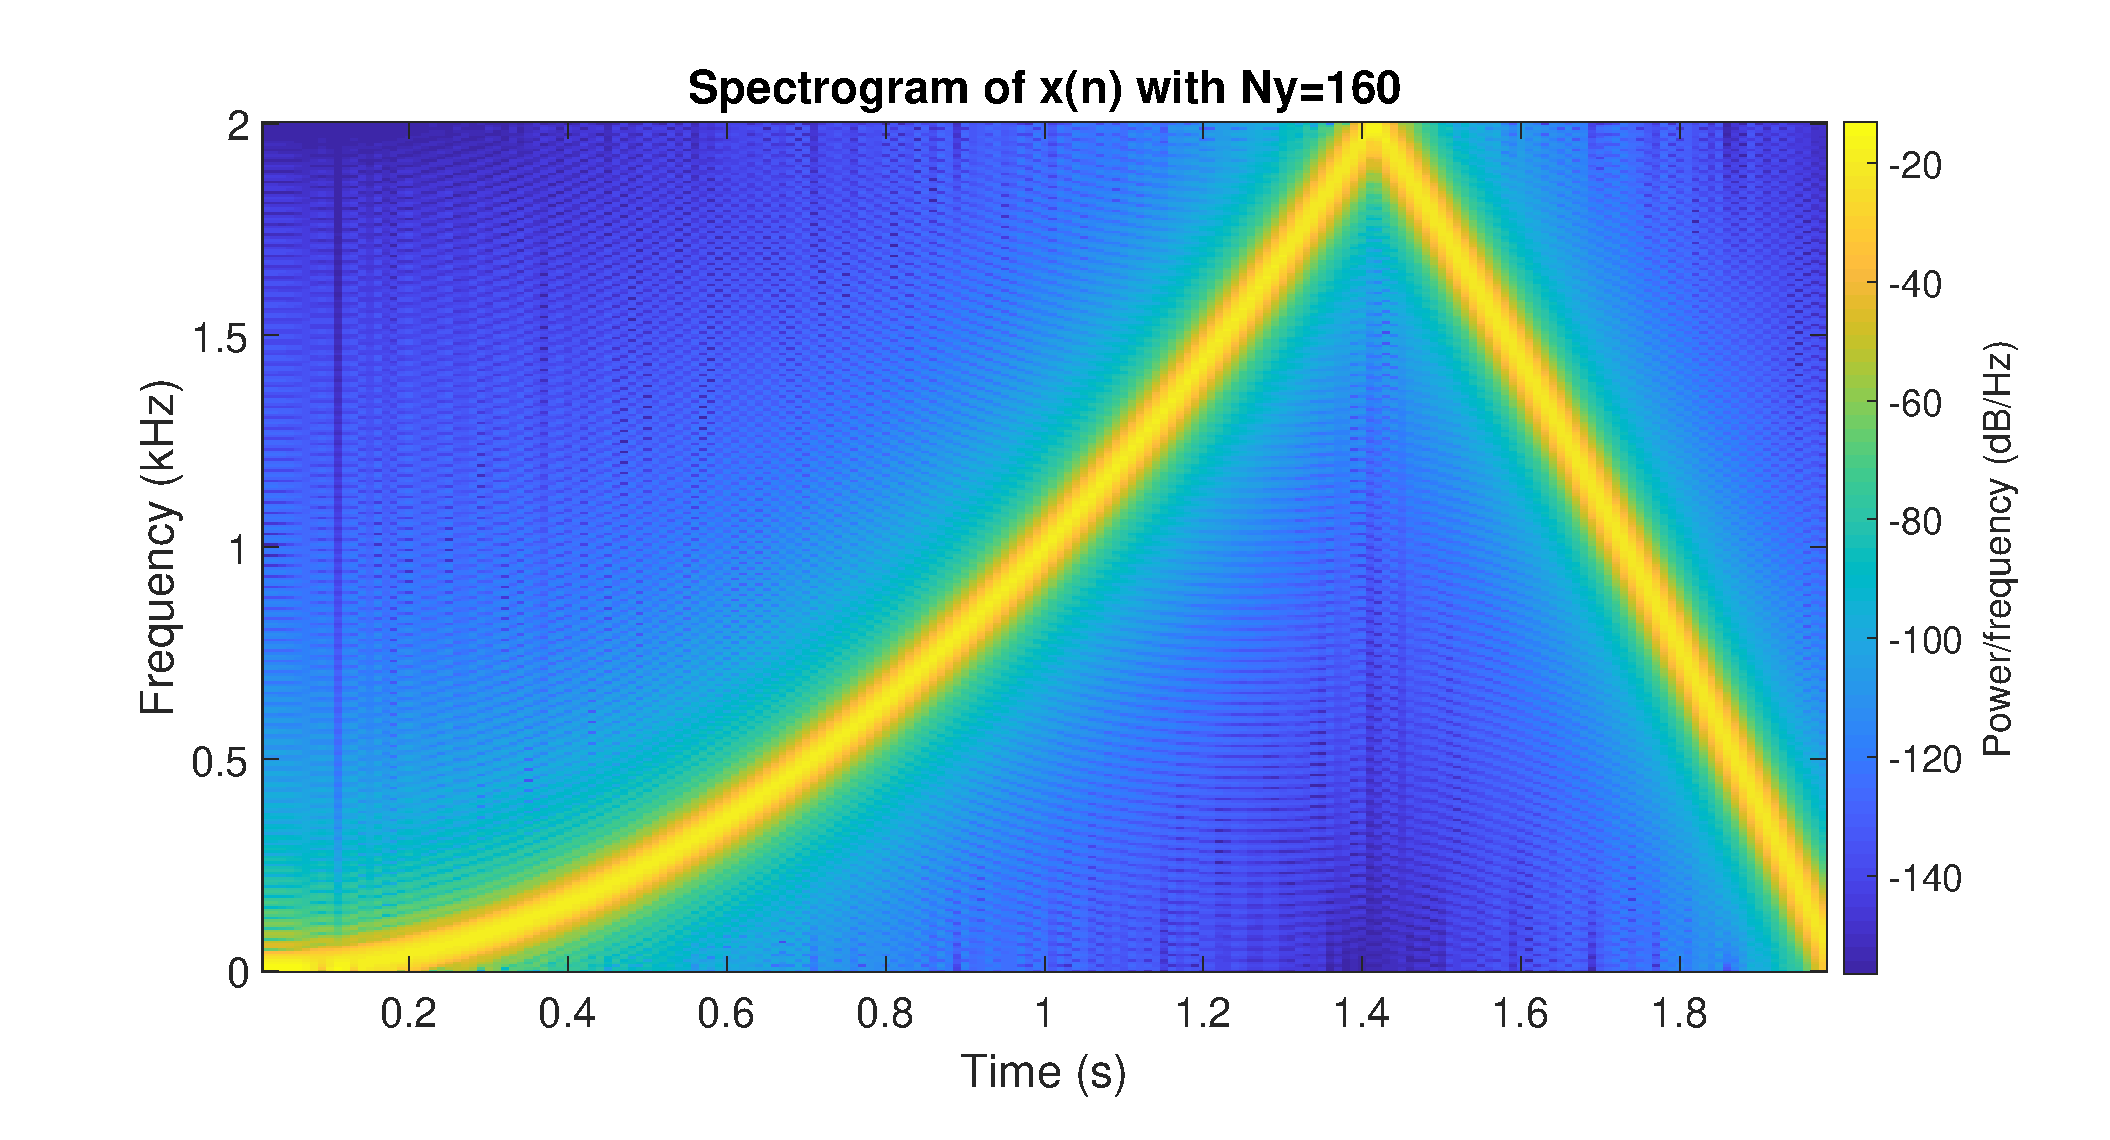
\includegraphics[width = 0.8 \textwidth]{figures/spectrogram_y.pdf}
    \caption{Spectrogram of $y(n)$ obtained with the MATLAB{\texttrademark} command \texttt{spectrogram} for an Hanning window with length $N_y = 160$, $3N_y/4$ overlapped samples, $4 N_y$ DFT points, and sampling frequency $f_s/2 = \SI{4000}{\hertz}$.}
    \label{fig:spectrogram_y}
\end{figure}

\subsection{3.c) Explanation of the aliasing phenomena}\label{sec:3c}

In order to further understand the aliasing phenomena, continuous-time signals $z_i: \mathbb{R} \rightarrow \mathbb{R}$, for $i = 1, ..., 4$ will be defined as
\begin{equation}
    z_i (t) = \cos ( 2 \pi f_i t),
\end{equation}
where $f_1 = \SI{1}{\kilo \hertz}$, $f_2 = \SI{2}{\kilo \hertz}$, $f_3 = \SI{3}{\kilo \hertz}$, and $f_4 = \SI{4}{\kilo \hertz}$. Sampling these signals at sampling frequencies $\SI{20}{\kilo \hertz}$, $\SI{8}{\kilo \hertz}$, and $\SI{4}{\kilo \hertz}$, one may obtain Fig. \ref{fig:z_1000} to \ref{fig:z_4000}. In Fig. \ref{fig:z_1000} and \ref{fig:z_2000}, it is possible to observe that the sampled signals have the frequency of the original continuous-time signal for all sampling frequencies. This is expected taking into account the Sampling Theorem. It is also visible that for the sampling frequency $\SI{4}{\kilo \hertz}$ and sinusoidal wave of frequency $\SI{2}{\kilo \hertz}$, the continuous-time signal is sampled precisely two times per period, which is the absolute minimum for sampling without distortion. In Fig. \ref{fig:z_3000}, there is already aliasing. The sampled signal has the frequency of the original continuous signal for the sampling frequencies $\SI{8}{\kilo \hertz}$ and $\SI{20}{\kilo \hertz}$ but, for the sampling frequency $\SI{4}{\kilo \hertz}$, the continuous signal completes 3 periods in the window considered, whereas the sampled signal completes only one. The frequency of the sampled signal is, thus, $\SI{1}{\kilo \hertz}$, indicating the presence of aliasing. In Fig. \ref{fig:z_4000}, there is aliasing at the same sampling frequencies. For the smallest sampling frequency, the sampled signal remains constant whereas the continuous signal completes 3 periods in the window considered. The frequency of the sampled signal is, thus, zero. From Fig. \ref{fig:z_3000} and \ref{fig:z_4000}, it is, thus, possible to interpret the distortion of the previous section. When a signal is sampled at a frequency higher than its highest frequency but smaller than twice its highest frequency, the frequencies are mapped into frequencies smaller than half the sampling frequency used. Furthermore, in this particular case, the higher the original frequency the lower it will be mapped, as it may be observed in Fig. \ref{fig:spectrogram_y}. This happens because its samples will slowly come to be made at the same instants of the period of the continuous-time signal at every of its periods. However, as one decreases the sampling frequency below the highest frequency of the signal, the frequency of the sampled signal begins to increase again as can be seen in Fig. \ref{fig:spectrogram_c} for a signal $c(n)$ sampled from $x_c(t)$ at half its highest frequency. This can be explained taking into consideration that, as the sampling frequency decreases, the samples will be taken at increasingly spaced instants inside the periods of the signals. Furthermore, one can state that this behaviour is cyclic and will repeat itself as the sampling frequency drops.

\begin{figure}[ht!]
    \centering
     \begin{subfigure}[b]{0.49\textwidth}
         \centering
         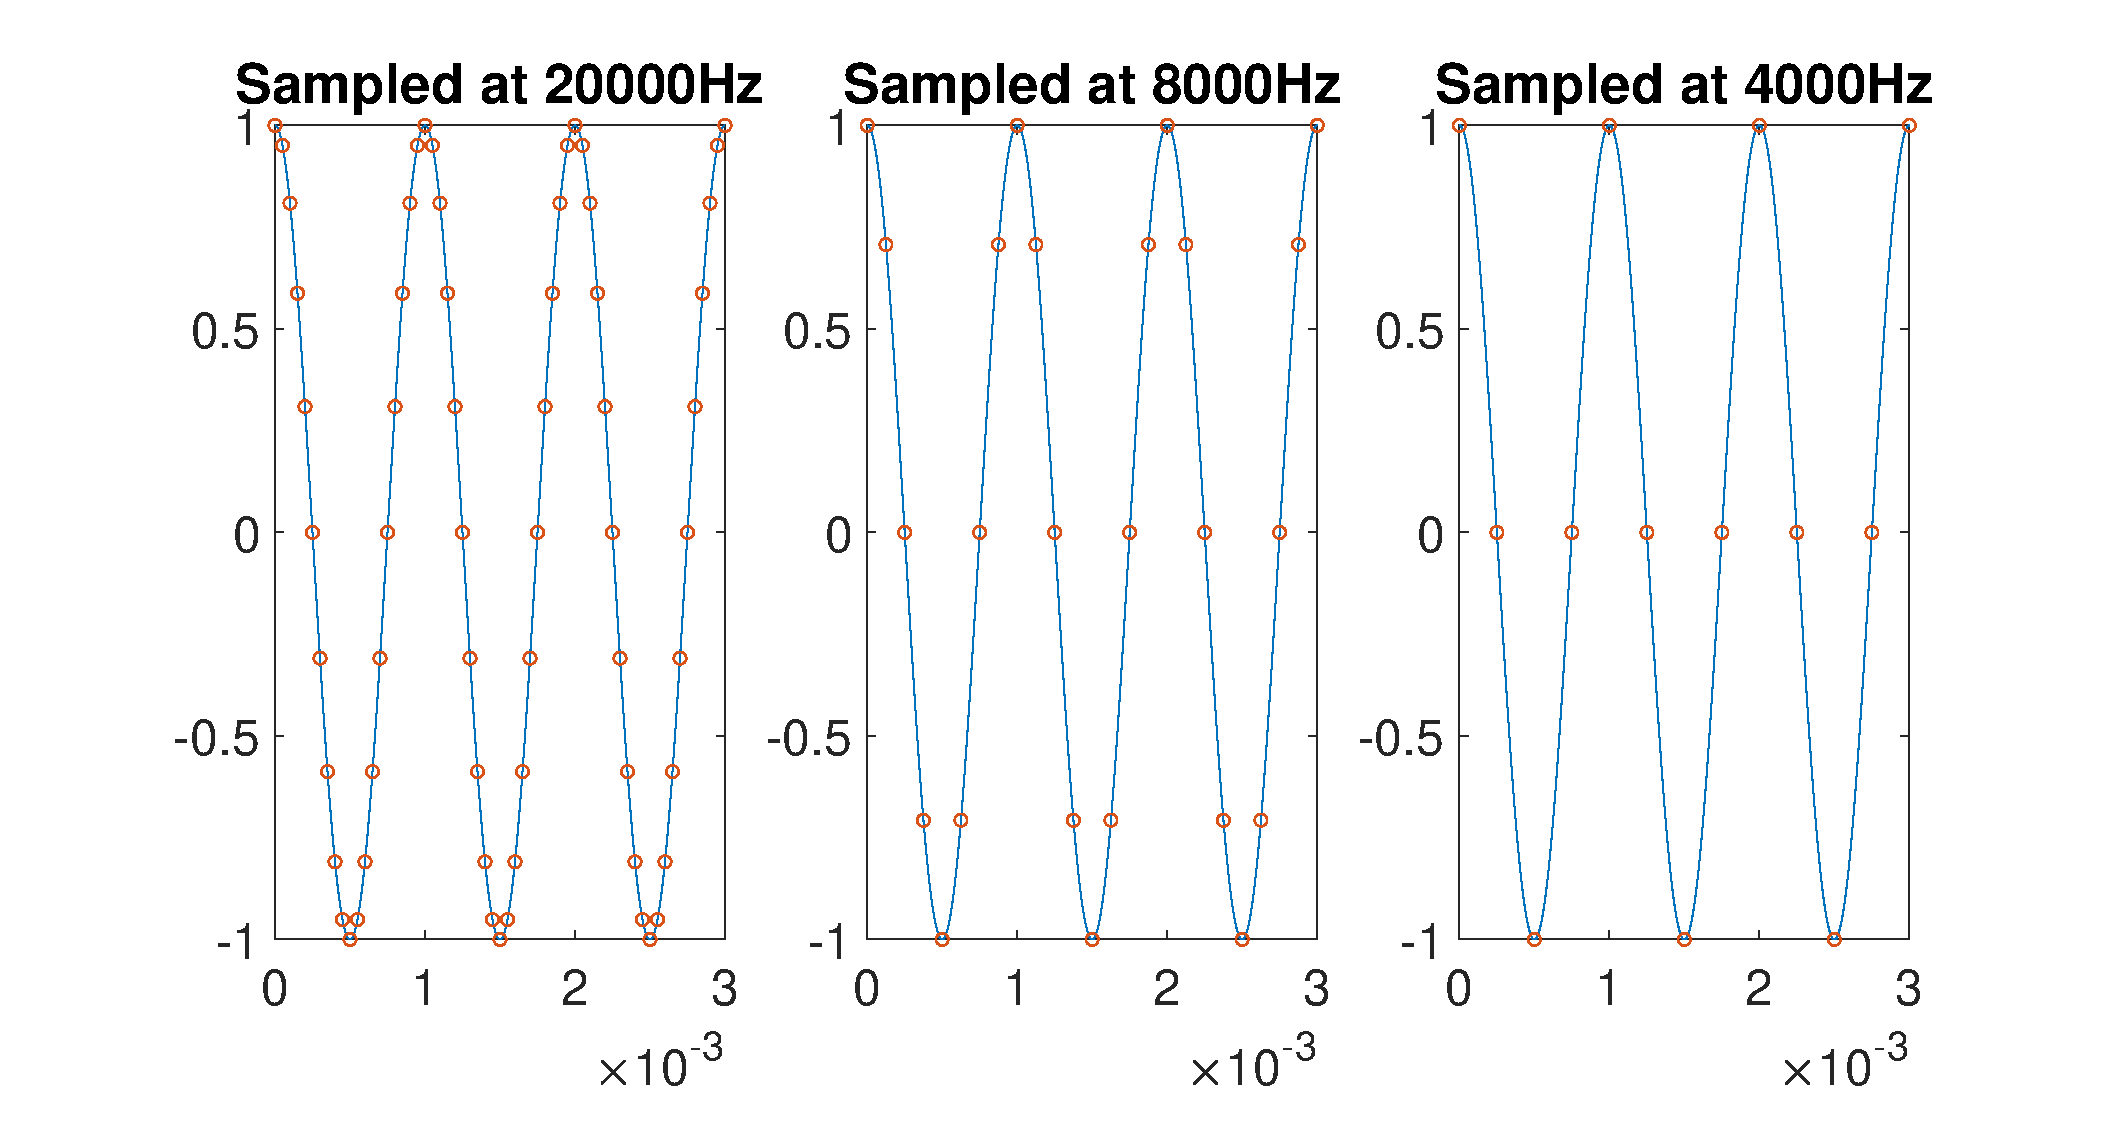
\includegraphics[width=\textwidth]{figures/plot_z_1000_Hz.pdf}
         \caption{Plot of the signal $z_1$ ($f_1 = \SI{1}{\kilo \hertz}$) overlapped with the corresponding sampled signal at different sample frequencies.}
         \label{fig:z_1000}
     \end{subfigure}
     \hfill
     \begin{subfigure}[b]{0.49\textwidth}
         \centering
         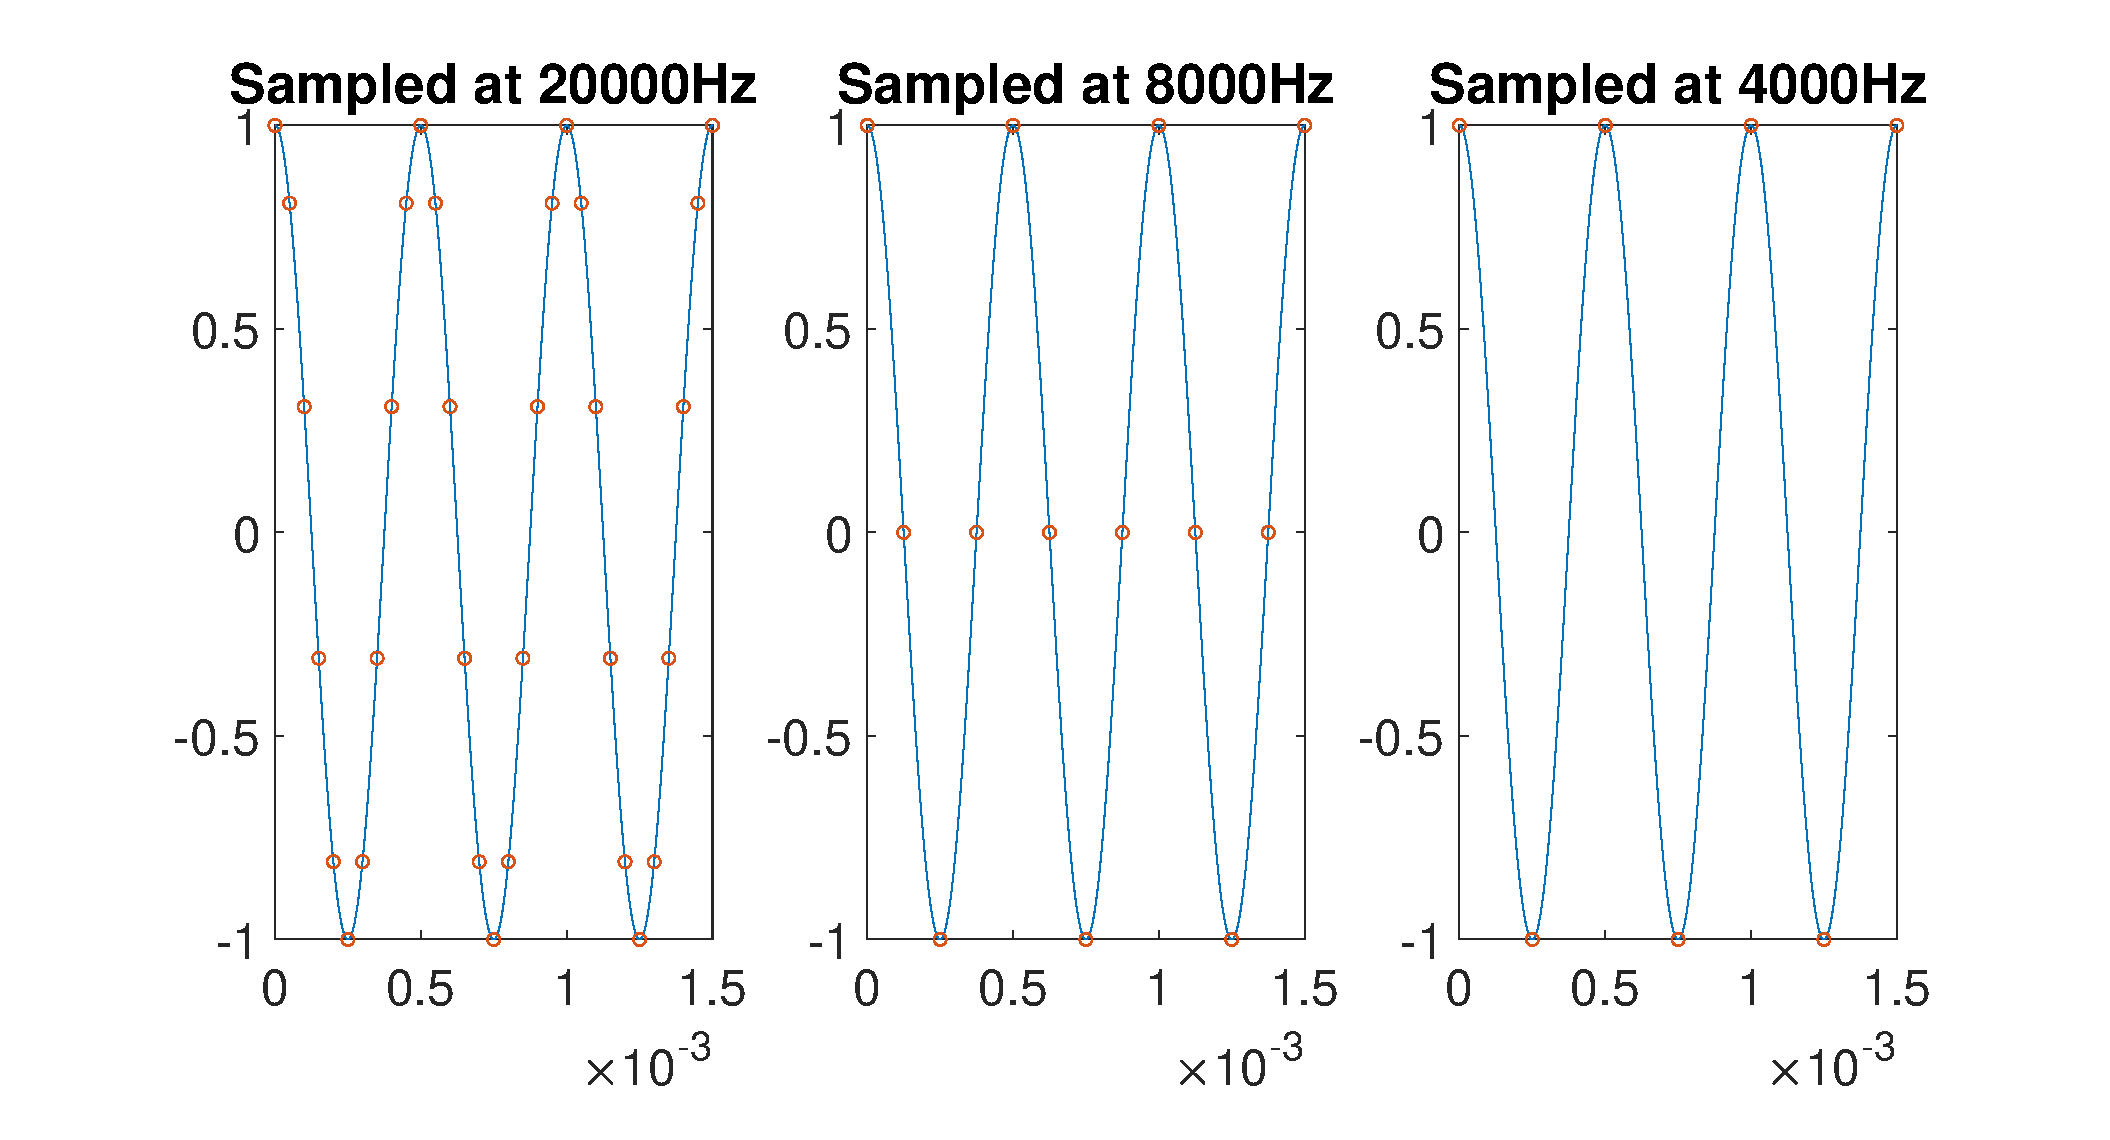
\includegraphics[width=\textwidth]{figures/plot_z_2000_Hz.pdf}
         \caption{Plot of the signal $z_2$ ($f_2 = \SI{2}{\kilo \hertz}$) overlapped with the corresponding sampled signal at different sample frequencies.}
         \label{fig:z_2000}
     \end{subfigure}
     \\
    \begin{subfigure}[b]{0.49\textwidth}
         \centering
         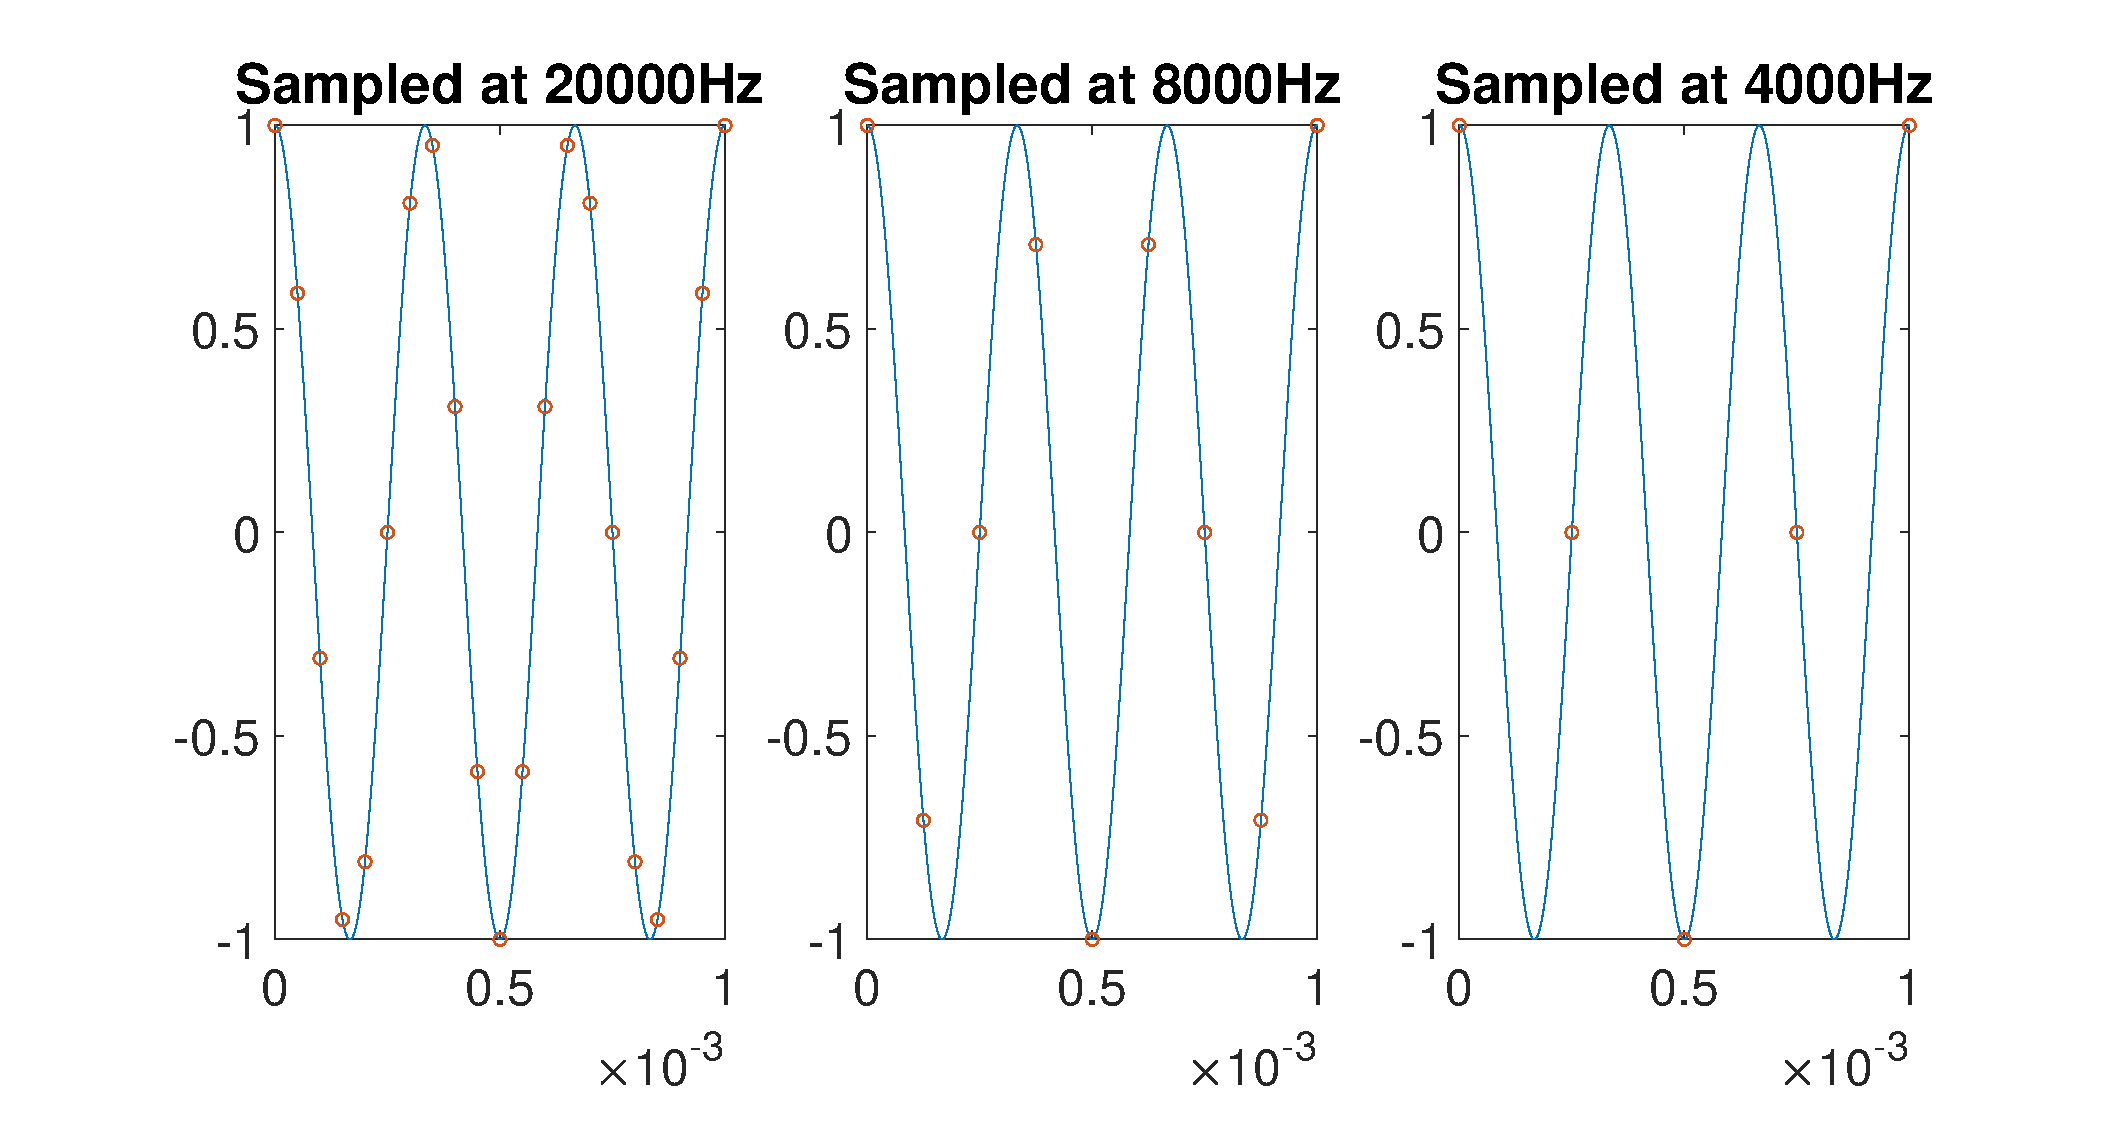
\includegraphics[width=\textwidth]{figures/plot_z_3000_Hz.pdf}
         \caption{Plot of the signal $z_3$ ($f_3 = \SI{3}{\kilo \hertz}$) overlapped with the corresponding sampled signal at different sample frequencies.}
         \label{fig:z_3000}
     \end{subfigure}
     \hfill
     \begin{subfigure}[b]{0.49\textwidth}
         \centering
         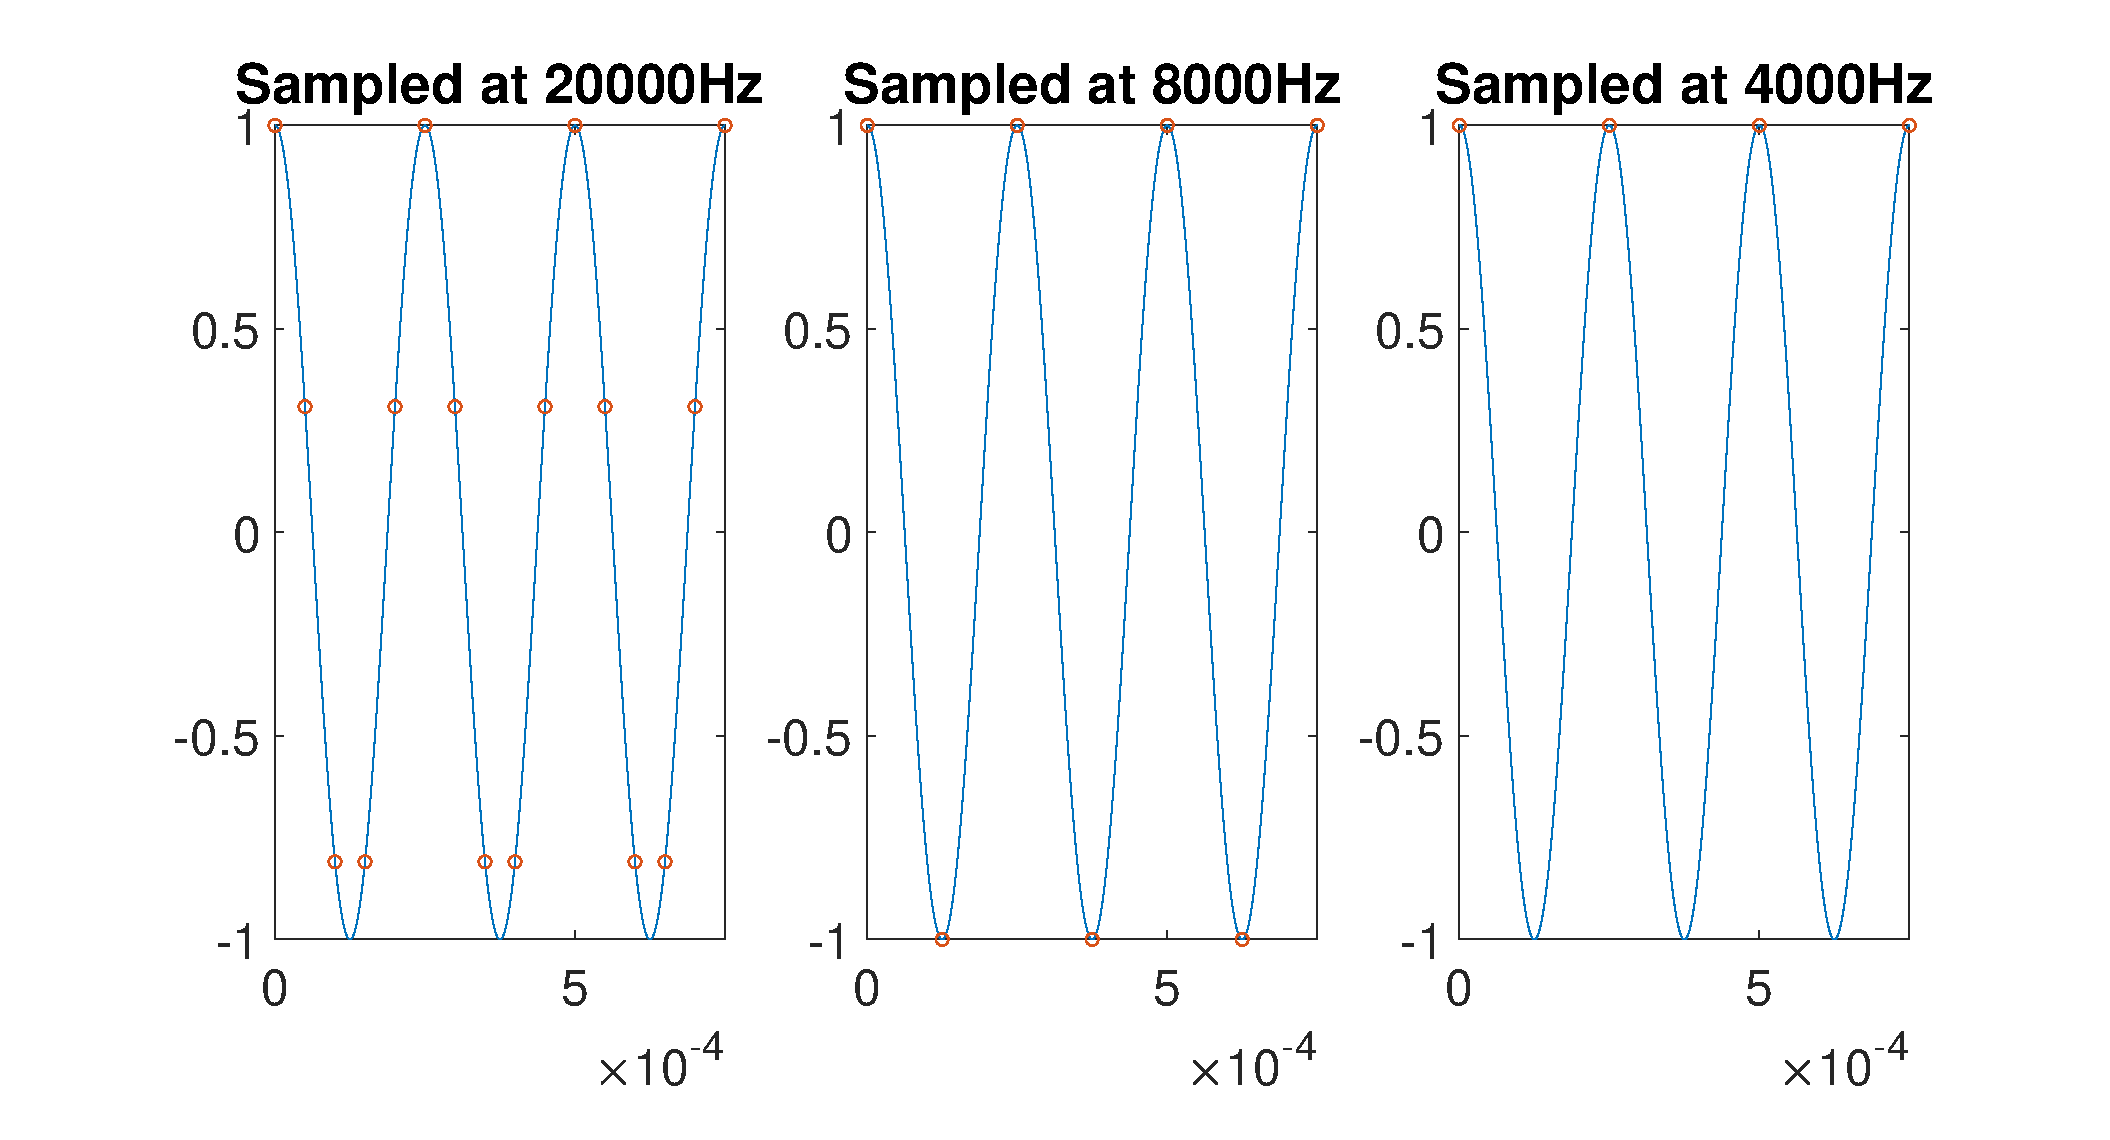
\includegraphics[width=\textwidth]{figures/plot_z_4000_Hz.pdf}
         \caption{Plot of the signal $z_4$ ($f_4 = \SI{4}{\kilo \hertz}$) overlapped with the corresponding sampled signal at different sample frequencies.}
         \label{fig:z_4000}
     \end{subfigure}
     \caption{Plots of the signals $z_i$ for different frequencies $f_i$ overlapped with the corresponding sampled signals at different sample frequencies.}
\end{figure}

\begin{figure}[ht!]
    \centering
    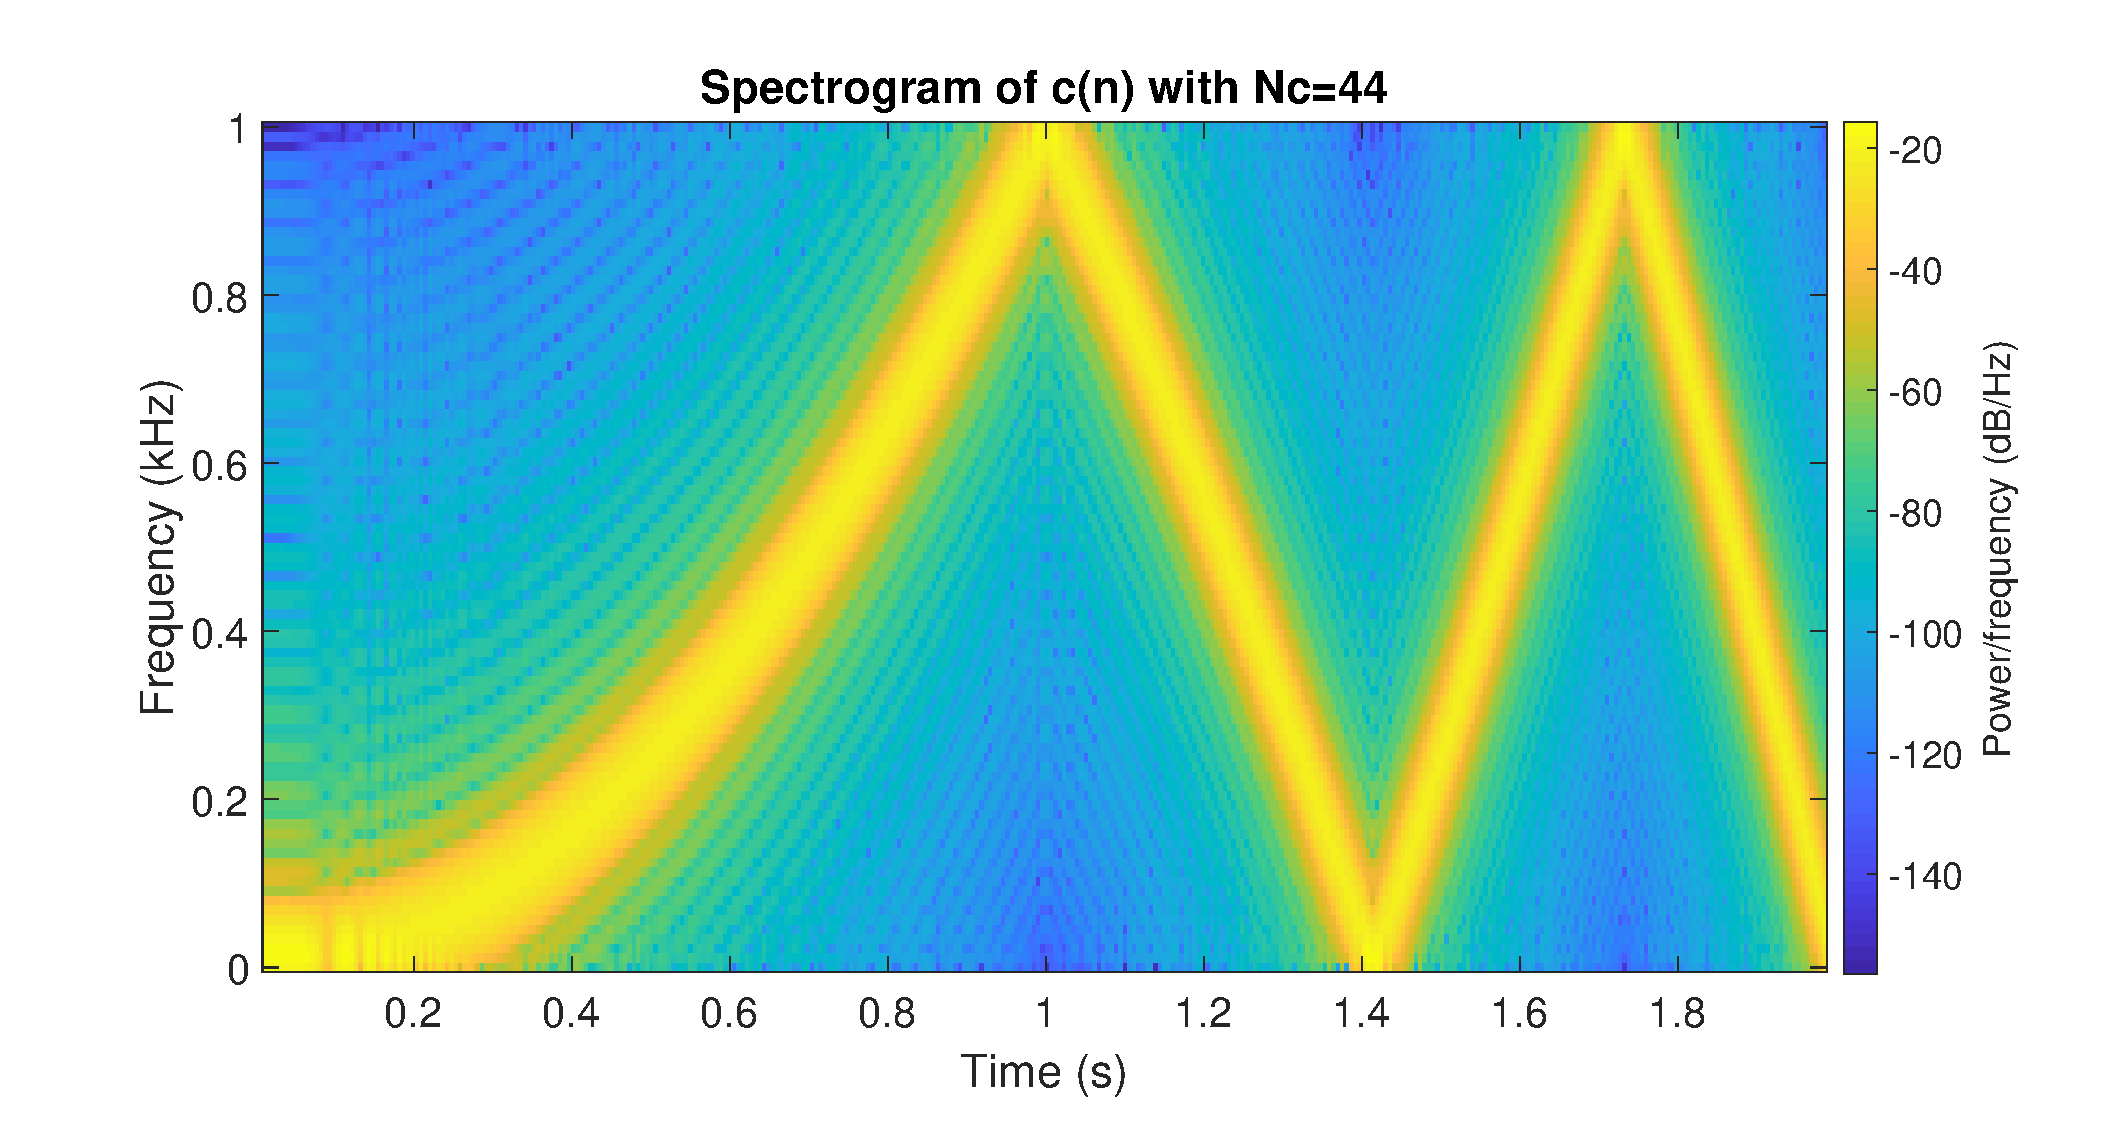
\includegraphics[width = 0.8 \textwidth]{figures/spectrogram_c.pdf}
    \caption{Spectrogram of $c(n)$ obtained with the MATLAB{\texttrademark} command \texttt{spectrogram} for an Hanning window with length $N_c = 44$, $3N_c/4$ overlapped samples, $4 N_c$ DFT points, and sampling frequency $f_s/4 = \SI{2000}{\hertz}$.}
    \label{fig:spectrogram_c}
\end{figure}

\newpage
\section{Romanza}

\subsection{4.a) Original sound signal}\label{sec:4}
The digital sound signal stored in the file {\texttt romanza\textunderscore pe.wav}, that was provided, was uploaded to MATLAB\texttrademark. It corresponds to the digitization of an original analog sound signal with a sampling rate of $f_s = 44.1$kHz. The digital signal plays a sharp melody of a violin playing. To analyze the digital sound signal in the frequency domain, its spectrogram was plotted. It is presented, for the first 15s of the signal, in Fig. \ref{fig:spctOriginal}, with a window of $N = 2400$ and sampling frequency $f_s = \SI{44.1}{\kilo \hertz}$. Whenever a certain note is played on the violin, the cords vibrate at a specific combination of harmonics, which are integer multiples of a fundamental frequency. In fact, these harmonics are noticeable in the spectrogram of Fig. \ref{fig:spctOriginal}.

\begin{figure}[h!]
	\centering
	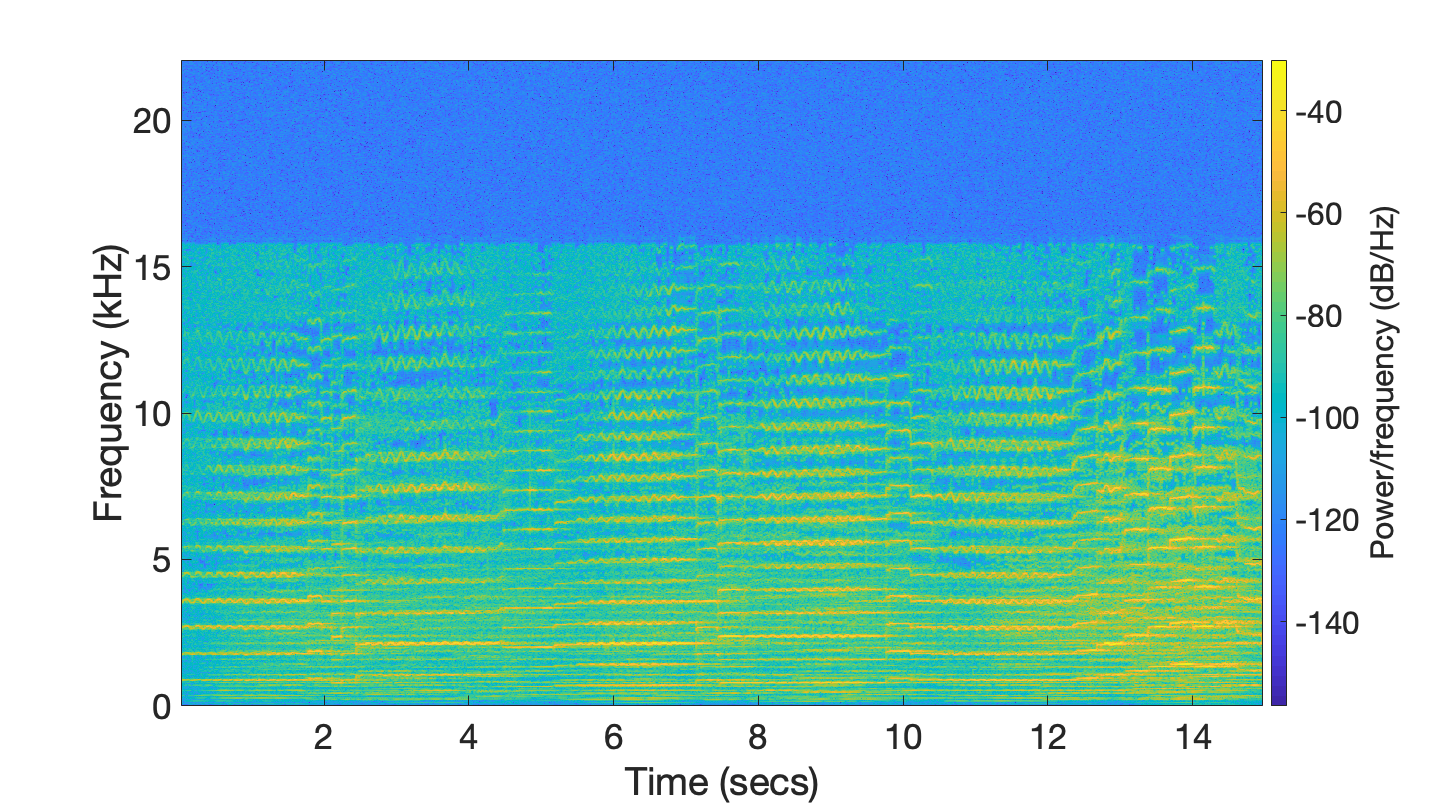
\includegraphics[width=0.8\textwidth]{figures/spect_original.png}
	\caption{Spectrogram of the original digital sound signal for the first 15s, with a window length of $N = 2400$ and sampling frequency $f_s = \SI{44.1}{\kilo \hertz}$.}
	\label{fig:spctOriginal}
\end{figure}

As a matter of fact, its is noticeable that there are some well defined time intervals for which the spectrogram is a set of approximately horizontal lines. These are integer multiples of the lowest frequency (the fundamental frequency) that defines the note being played on the violin. As an illustrative example, from $t=0$s to $t=1.7$s, the spectrogram is a set of approximately horizontal lines at frequencies which are integer multiples of $f_0 \approx 877.5$Hz. It is, thus, possible to conclude that the note played in this interval is A5, \textit{i.e.}, note A (\textit{lá} in Portuguese) of the fifth octave, which has a fundamental frequency $f_{A5} = 880$Hz.

\subsection{5.a) Sampling at a 1/5 of the original rate}\label{sec:5}
From the original digital signal, a new digital signal was obtained corresponding to the signal that would be obtained if the original analog sound signal was sampled at a fifth of the rate at which it is sampled in the file {\texttt romanza\textunderscore pe.wav}. That is, the new signal was obtained with a sampling rate $f_{s_5} = f_s/5 = 8.82$kHz.

The digital signal plays a somewhat unpleasant sound of a violin playing. Although it is still possible to identify the melody played in Section \ref{sec:4}, it is significantly distorted. To analyze the digital sound signal in the frequency domain and identify the source of the distortion heard, its spectrogram was plotted. It is presented, for the first 15s of the signal, in Fig. \ref{fig:spect_5}, with sampling frequency $f_{s_5} = \SI{8.82}{\kilo \hertz}$ and a window length $N = 2400/5=480$, so that the window duration is maintained.

\begin{figure}[h!]
	\centering
	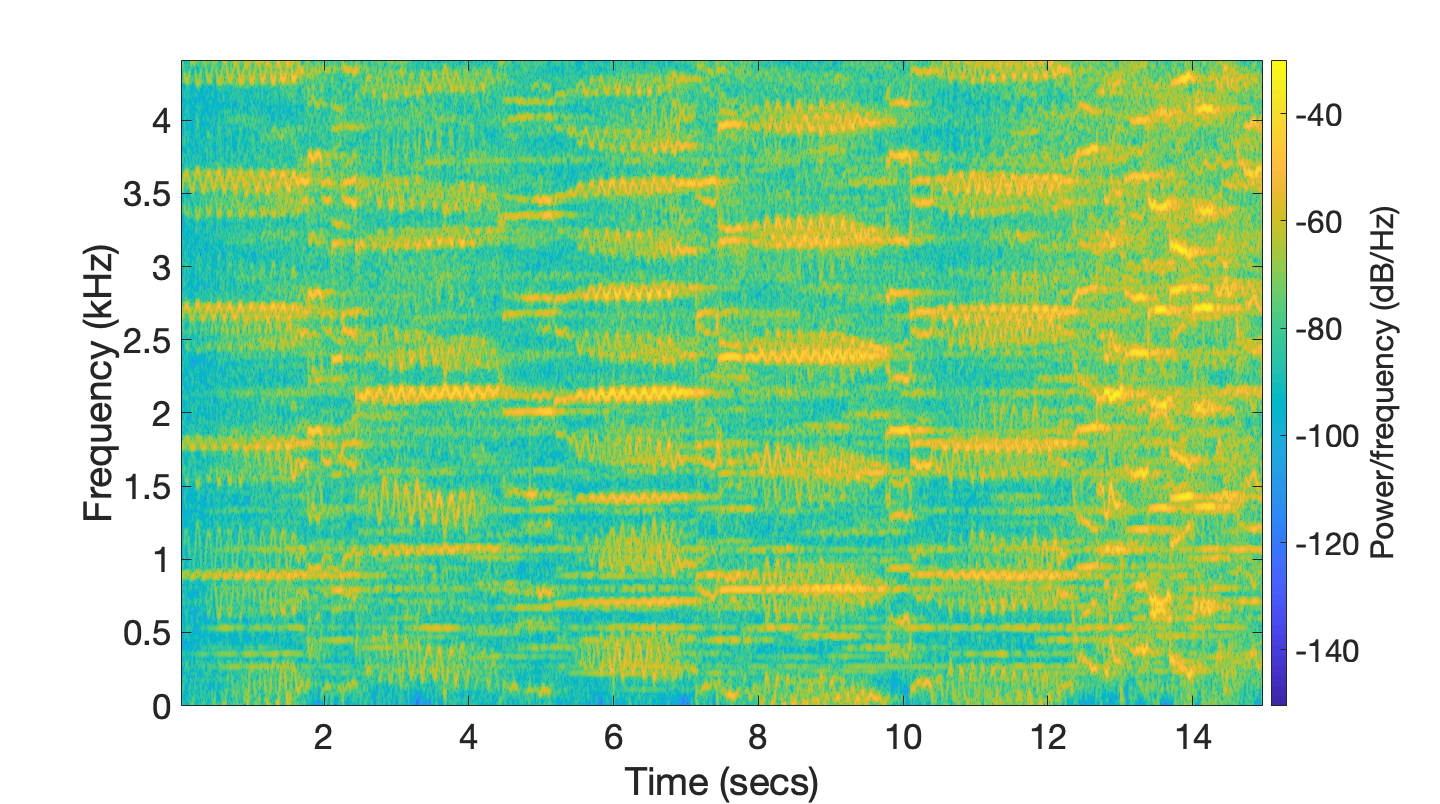
\includegraphics[width=0.8\textwidth]{figures/spect_5.png}
	\caption{Spectrogram of the original sound signal obtained in 5, for the first 15s, with a window of $N = 480$ and sampling frequency $f_{s_5} = \SI{8.82}{\kilo \hertz}$.}
	\label{fig:spect_5}
\end{figure}

The lower frequencies of the original song appear to be played as they were in the original audio signal. However, the higher frequencies are no longer heard and, as displayed in the spectrogram, they are distorted (given that they are no longer multiples of the fundamental frequency) and played as lower frequencies. This phenomenon is due to the fact that it is not possible to identify any frequencies above half the sampling frequency $f_{s_5}/2 = 4.41$kHz, as expected from the Sampling Theorem. These frequencies are mapped into the interval $[0; f_{s_5}/2]$, as discussed in Section \ref{sec:3c}, and distort the signal that is heard. Nevertheless, it is still possible to identify some harmonics of the violin, despite the fact that they are superimposed with the distorted higher frequencies. This is only possible because the fundamental frequency of the notes played on the violin is below half the new sampling frequency.

\subsection{6.a) Sampling at a 1/5 of the original rate after filtering}\label{sec:6}

In this subsection, the original digital signal is filtered in a first instance. The filtering stage is carried out using a order 100 low-pass FIR filter with cut-off frequency $\omega_{co} = 0.2 \pi \; \mathrm{rad\:s^{-1}}$, in the angular-frequency scale of the discrete-time Fourier transform. In continuous-time the cut-off frequency corresponds to $f_{co} = \Omega_{co}/(2\pi) =  \omega_{co} f_s /(2\pi) = 4.41$kHz. It is important to remark that $f_{co} = f_{s_5}/2$. The spectrogram of the filtered signal is presented in Fig. \ref{fig:spect_6_filt}. It is possible to see in this plot that the harmonics with a frequency above $f_{co}$ are highly attenuated. The filtered signal is then sampled at a sampling rate of $f_{s_5}= 8.82$kHz.

\begin{figure}[h!]
	\centering
	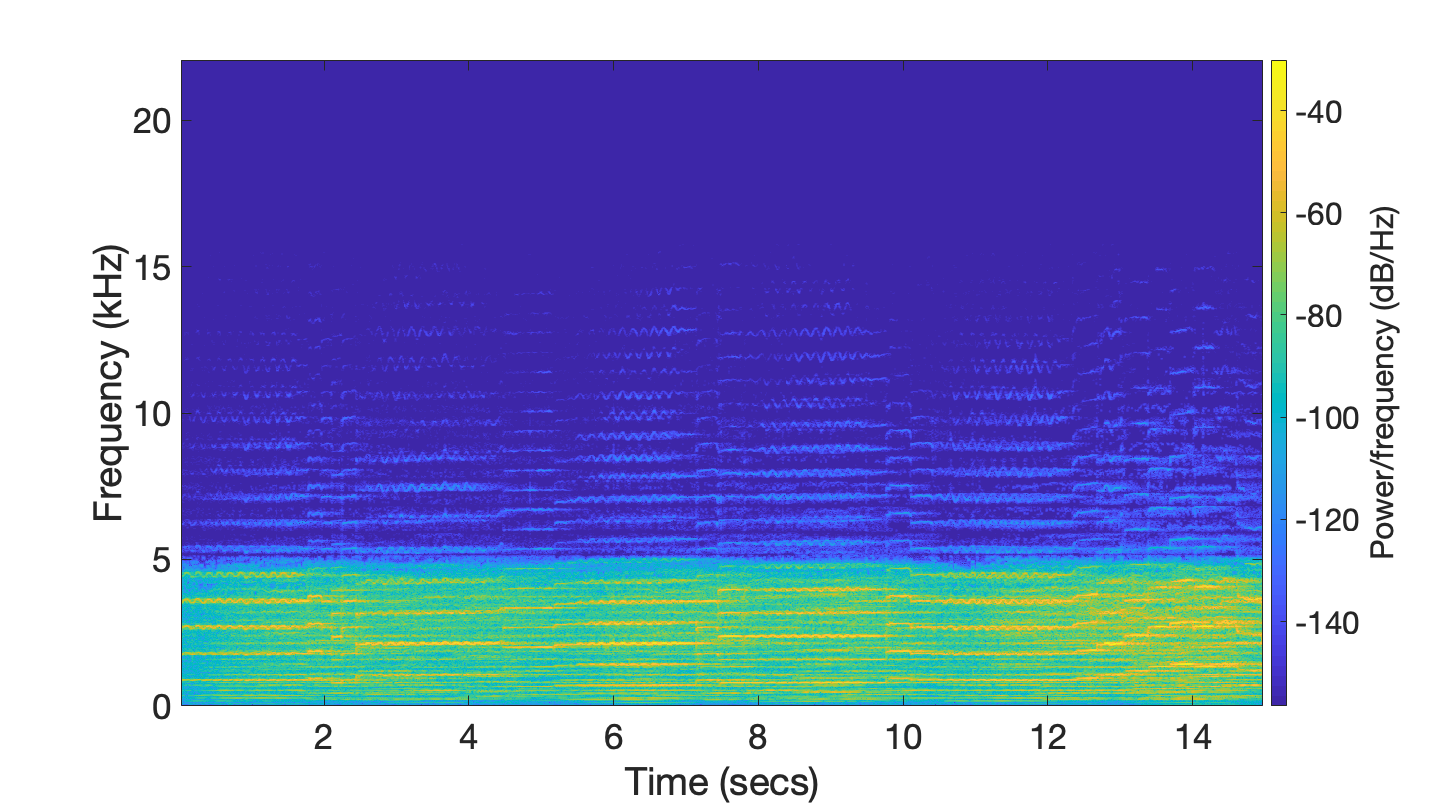
\includegraphics[width=0.8\textwidth]{figures/spect_6_filt.png}
	\caption{Spectrogram of the filtered signal, for the first 15s, with a window of $N = 2400$.}
	\label{fig:spect_6_filt}
\end{figure}

The new digital signal plays a pleasant undistorted melody of a violin playing, contrarily to what was heard in Section \ref{sec:5}. To analyze the digital sound signal in the frequency domain and understand why, unlike the signal sampled in Section \ref{sec:5}, the signal is undistorted, its spectrogram was plotted. It is presented, for the first 15s of the signal, in Fig. \ref{fig:spect_6}, with a window length $N = 2400/5=480$, again to maintain the window duration.

\begin{figure}[h!]
	\centering
	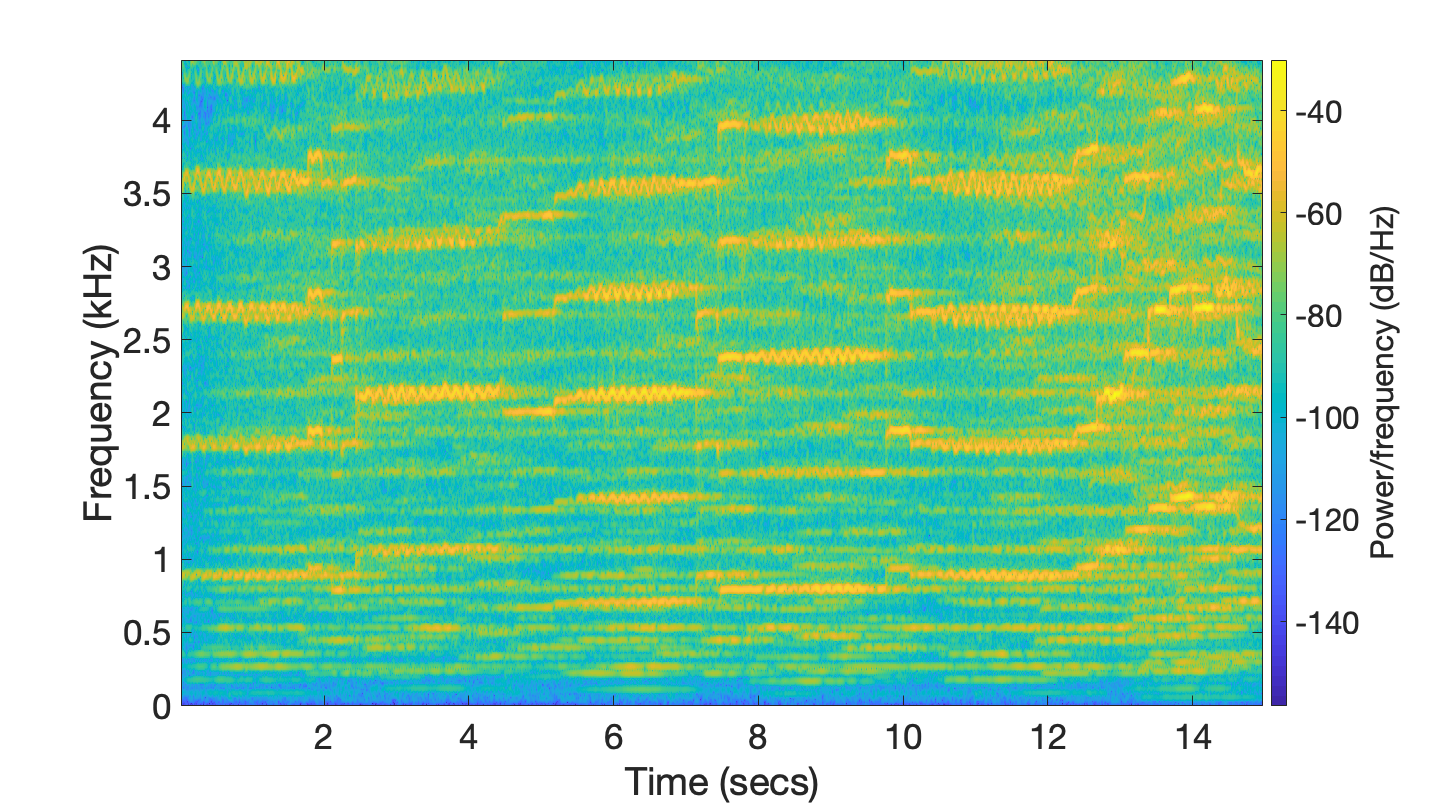
\includegraphics[width=0.8\textwidth]{figures/spect_6.png}
	\caption{Spectrogram of the sound signal obtained in 6, for the first 15s, with a window length of $N = 480$.}
	\label{fig:spect_6}
\end{figure}

First, hearing the new sampled signal, which was filtered beforehand, and comparing it with the original song, it is evident that the higher frequencies are no longer heard. In fact, given that the filter has a high order and cut-off frequency $f_{co} = 4.41$kHz, it is expected that frequencies above it are highly attenuated, as seen in Fig. \ref{fig:spect_6_filt}, and, thus, no longer heard. Second, note that the cut-off frequency of the low-pass FIR filter corresponds to the highest frequency that it is possible to identify with the sampling rate $f_{s_5}$, which is, from the Sampling Theorem, $f_{s_5}/2 = 4.41\mathrm{kHz} = f_{co}$. Third, note that although the signals obtained in Sections \ref{sec:5} and \ref{sec:6} are sampled at the same rate, the former is distorted but the latter is not. In fact, whereas in Section \ref{sec:5} the signal that was sampled contained frequencies higher that half the sampling frequency, in Section \ref{sec:6} the signal that was sampled does not because they were attenuated beforehand by the FIR filter. For this reason, while the signal obtained in Section \ref{sec:5} sounds very distorted, the sound played by the signal obtained in Section \ref{sec:6} does not. Fourth, the previously detailed difference is also noticeable comparing the spectrograms in Figs. \ref{fig:spect_5} and \ref{fig:spect_6}. In fact, whereas in the spectrogram in Fig. \ref{fig:spect_5} the low frequency harmonics are superimposed with the distorted high frequency harmonics of the original song, in the spectrogram in Fig. \ref{fig:spect_6} the low frequency harmonics are easily detected and are prominent, presenting very little distortion. It is also interesting to point out that, albeit very attenuated by the FIR filter, the higher frequencies mapped into the interval $[0; f_{s_5}/2]$ are still noticeable in the faint green horizontal lines of Fig. \ref{fig:spect_6}. Fifth, the harmonics observed in Fig. \ref{fig:spect_6} correspond to multiples of the same fundamental frequency of the note played on the violin in the original signal. Thus, even though the original high frequency harmonics are filtered, it is possible to hear the same notes without distortion. As a result, even thought some sharpness is lost due to the filtering of the high frequencies, the melody is pleasant. Sixth, given the aforementioned aspects, suppose that it is necessary to sample a signal at a given sampling frequency. If such sampling frequency is lower than twice the highest frequency of that signal,  then, the original signal should be filtered before being sampled. Furthermore, the filter should be selected to be a low pass-filter with a cut-off frequency of half the sampling rate, in order to avoid distortion. 

\section{Conclusion}
In this laboratory it was possible to analyse and understand the effects of aliasing as a consequence of undersampling. In a first instance, the sampling of a chirp was analyzed as a means of understanding the causes of aliasing, as well as verifying the Sampling Theorem. In a second instance, an audio file of a violin playing was studied. It was possible to identify the harmonics of each note played. It was verified that, if the signal is sampled below the Nyquist frequency, the harmonics below the Nyquist frequency are mapped into a lower frequency and distort the note played. Finally, it was possible to conclude that, if it is necessary to use a sampling frequency that is lower than twice the highest frequency of a signal, then, the original signal should be filtered before being sampled with a low pass-filter with a cut-off frequency of half the sampling rate, in order to avoid distortion.
\end{document}
